%% V1.0
%% by Gabriel Garcia, gabrcg@gmail.com
%% This is a template for Udacity projects using IEEEtran.cls

%% Be Udacious!

\documentclass[10pt,journal,compsoc]{IEEEtran}

\usepackage[pdftex]{graphicx}    
\usepackage{cite}
\usepackage{tikz,pgfplots,filecontents}
\usepackage{pgfplots}
\usepackage{pgfplotstable}

\begin{document}

\title{APPROXIMATION on the ORBITIAL PARAMETER of NN SERPENTIS}

\author{KaChun Chan\\Department of Physics, University of California, Santa Barbara, CA 93106}



{}
\IEEEtitleabstractindextext{%

\begin{abstract}
\\Me and my lab partner used source extractor to extract data from three hundred and two fits images on NN Serpentis. Within these data, we took all the apparent magnitude, m, as well as its uncertainty, on 7th May,2014. However, these apparent magnitude has a offset.Therefore, we did our calibration by comparing our data to SIMBAD Astronomical Database. We then were able to display the relation between apparent magnitude and time. This allow us to measure the period of the orbital, as well as some useful parameter. Although NN Serpentis is a binary system, we can still treat it as a circular motion system due to the sine like relation between magnitude and time (see discussion section for detail explanation). We were able to derive some simple formula by apply the physics of circular motion and the physics of a white dwarf, which allow us to approximate the mass and radius of the white dwarf in NN Serpentis. Some of our results are accurate, but some of orbital parameters are off by a few factor to a factor of 10.
\end{abstract}

% Note that keywords are not normally used for peerreview papers.
\begin{IEEEkeywords}
NN Serpentis, Radius, Mass, White Dwarf, Orbital Parameter
\end{IEEEkeywords}}


\maketitle
\IEEEdisplaynontitleabstractindextext
\IEEEpeerreviewmaketitle
\section{Introduction}
\label{sec:introduction}

\IEEEPARstart
 {}
\\NN Serpentis is a binary system composed with a white dwarf and red dwarf that orbiting each other. They share the same  Right Ascension and Declination due to the far distance from earth, which are 15h 52m 56.131s and +12° 54′ 44.68 respectively [2]. Binary system is a system that consists of two star orbiting around the common center, which is not necessary to be a circular path. However, in our case, we can reasonably assume that that orbit is circular with the data on apparent magnitude (see discussion section for detail explanation).Since the white dwarf and the red dwarf are orbiting each other, the apparent magnitude is a function of time. By plotting the relation, we were able to find the orbiting period and the eclipse time
\\A white dwarf is a star that had gone through both hydrogen and helium burning phase, and starts burning carbon. The white dwarf is also a dense star which support by the pressure. The mass- radius relation of a white dwarf is \begin{equation}
R\approx\frac{R_\odot}{74}\Big[\frac{M_\odot}{M}\Big]^{1/3}
\end{equation}
\\where $R_\odot$ and $M_\odot$ are the solar radius and the solar mass respectively. Such relation is only applicable to low mass white dwarfs [3].
\\The apparent magnitude is essentially related to the brightness. It plays a key role in the determination of the orbital period. The apparent magnitude has a sine like relation with time. A complete sine curve is correspond to a full orbit. Thus, the eclipse will be shown on the apparent magnitude vs time curve, which allow us to calculate the radius and the mass of the white dwarf, as well as the orbital radius of NN Serpentis with the formula we have derived.
\\On the other hand, by citing the absolute magnitude from online data base, we will be able to calculate the distance from the Earth to the NN Serpentis. The relation between the apparent magnitude, m, and the absolute magnitude, M, of the same object is 
\begin{equation}
m - M = 5logr - 5
\end{equation} 
\\where r is the actual distance to the white dwarf in parsecs [4]. According to the , the absolute magnitude is 8.11 [5].
\\NN Serpentis has a circular orbit, so we have the following relation,
\begin{equation}
F_{gravity}=\frac{Gm_w m_r}{d^{2}}
\end{equation}
\begin{equation}
F_{centripetal}=\frac{m_r v^{2}}{d}
\end{equation}
\\where $m_w$, $m_r$,$v$ and $d$ are the mass of white dwarf, the mass of red dwarf, the orbital speed and the orbital radius. We can then combine the gravitational force with the centripetal force. We will get 
\begin{equation}
\frac{Gm_w}{d}=v^{2}
\end{equation}
Replace the orbital speed, v, by the orbital period, T. We have
\begin{equation}
\frac{Gm_w}{d^{3}}=\frac{4\pi^{2}}{T^{2}}
\end{equation}




\begin{table*}[h!]
\centering
\caption{Data of selected stars}
\begin{tabular}{||c c c c c c c||} 
 \hline
 x(in pixel) & y(in pixel) & $Mag_{iso}$ & $Mag_{aper}$ & $MagB_{SIMBAD}$ & RA dec & ${Mag_{BSIMBAD} - Mag_{iso}}$ \\ [1ex] 
 \hline\hline
 865.841 & 1292.538 & -11.902 & -10.255 & 14.635[$\sim$] & 15 53 00.48 +12 52 35.7 & 26.537\\ 
 1002.905 & 1024.405 & -8.963 & -7.284 & 16[$\sim$] & 15 52 56.19 +12 54 47.4 & 24.963\\
 1247.278 & 796.237 & -12.951 & -11.061 & 13.762[$\sim$] & 15 52 48.22 +12 56 25.0 & 26.713\\
 1047.817 & 1215.368 & -11.654 & -10.047 & 15.136[$\sim$] & 15 52 54.67 +12 53 11.0 & 26.79\\
 1005.856 & 1250.534 & -11.887 & -10.25 & 16[$\sim$] & 15 52 56.06 +12 52 53.9 & 27.887\\
 1072.856 & 1012.77 & -10.48 & -8.912 & - & 15 52 53.79 +12 54 46.4 & -\\
 918.697  & 1745.861 & -11.687 & -9.99 & 12.3[0.26] & 15 52 58.90 +12 49 02.2 & 23.987\\
 672.412  & 1906.197 & -11.959 & -10.261 & 12.3[$\sim$] & 15 53 06.83 +12 47 45.9 & 24.259\\
 775.676  & 963.4 & -9.432 & -9.432 & 16.882[$\sim$] & 15 53 03.39 +12 55 09.6 & 26.314\\
 811.549 & 1780.664 & -12.111 & -7.443 & 12.3[$\sim$] & 15 53 02.36 +12 48 45.3 & 24.411\\
 784.116 & 1831.863 & -13.958 & -12.255 & 11.3[$\sim$] & 15 53 03.24 +12 48 21.1 & 25.258\\[1ex] 
 \hline
\end{tabular}
\label{table:1}
\end{table*}

\begin{table*}[h!]
\centering
\begin{tabular}{|c c|}
\hline
Average offset on Apparent Magnitude & Uncertainty \\  [1 ex] \hline\hline
25.7119 & 0.026 \\ [1ex]\hline
\end{tabular}
\end{table*}
\begin{table*}[h!]
\centering
\caption{stars position from one of the image}
\begin{tabular}{||c c c c c ||} 
 \hline 
 star & x(in pixel) & y(in pixel) & $Mag_{iso}$ & $Mag_{iso}+25.7119$ \\ [1ex]
 1 & 261.979 & 618.062 & -12.324 &13.3879\\
 2 & 1237.345 & 805.027 & -12.667 & 13.0449\\
 3 & 855.659 & 1301.142 & -11.903 & 13.8089\\
 4 & 1141.232 & 1602.256 & -11.527 & 14.1849\\
 5 & 775 & 1840.547 & -13.956 & 11.7569 \\[1ex] 
 \hline
\end{tabular}
\begin{tabular}{|| c||} 
 \hline
 Sum of the apparent magnitude ratio \\[1ex]
66.1835
\\[1ex] 
 \hline
\end{tabular}
\end{table*}
\begin{figure*}
\label{figure 1 - apparent magnitude vs time}
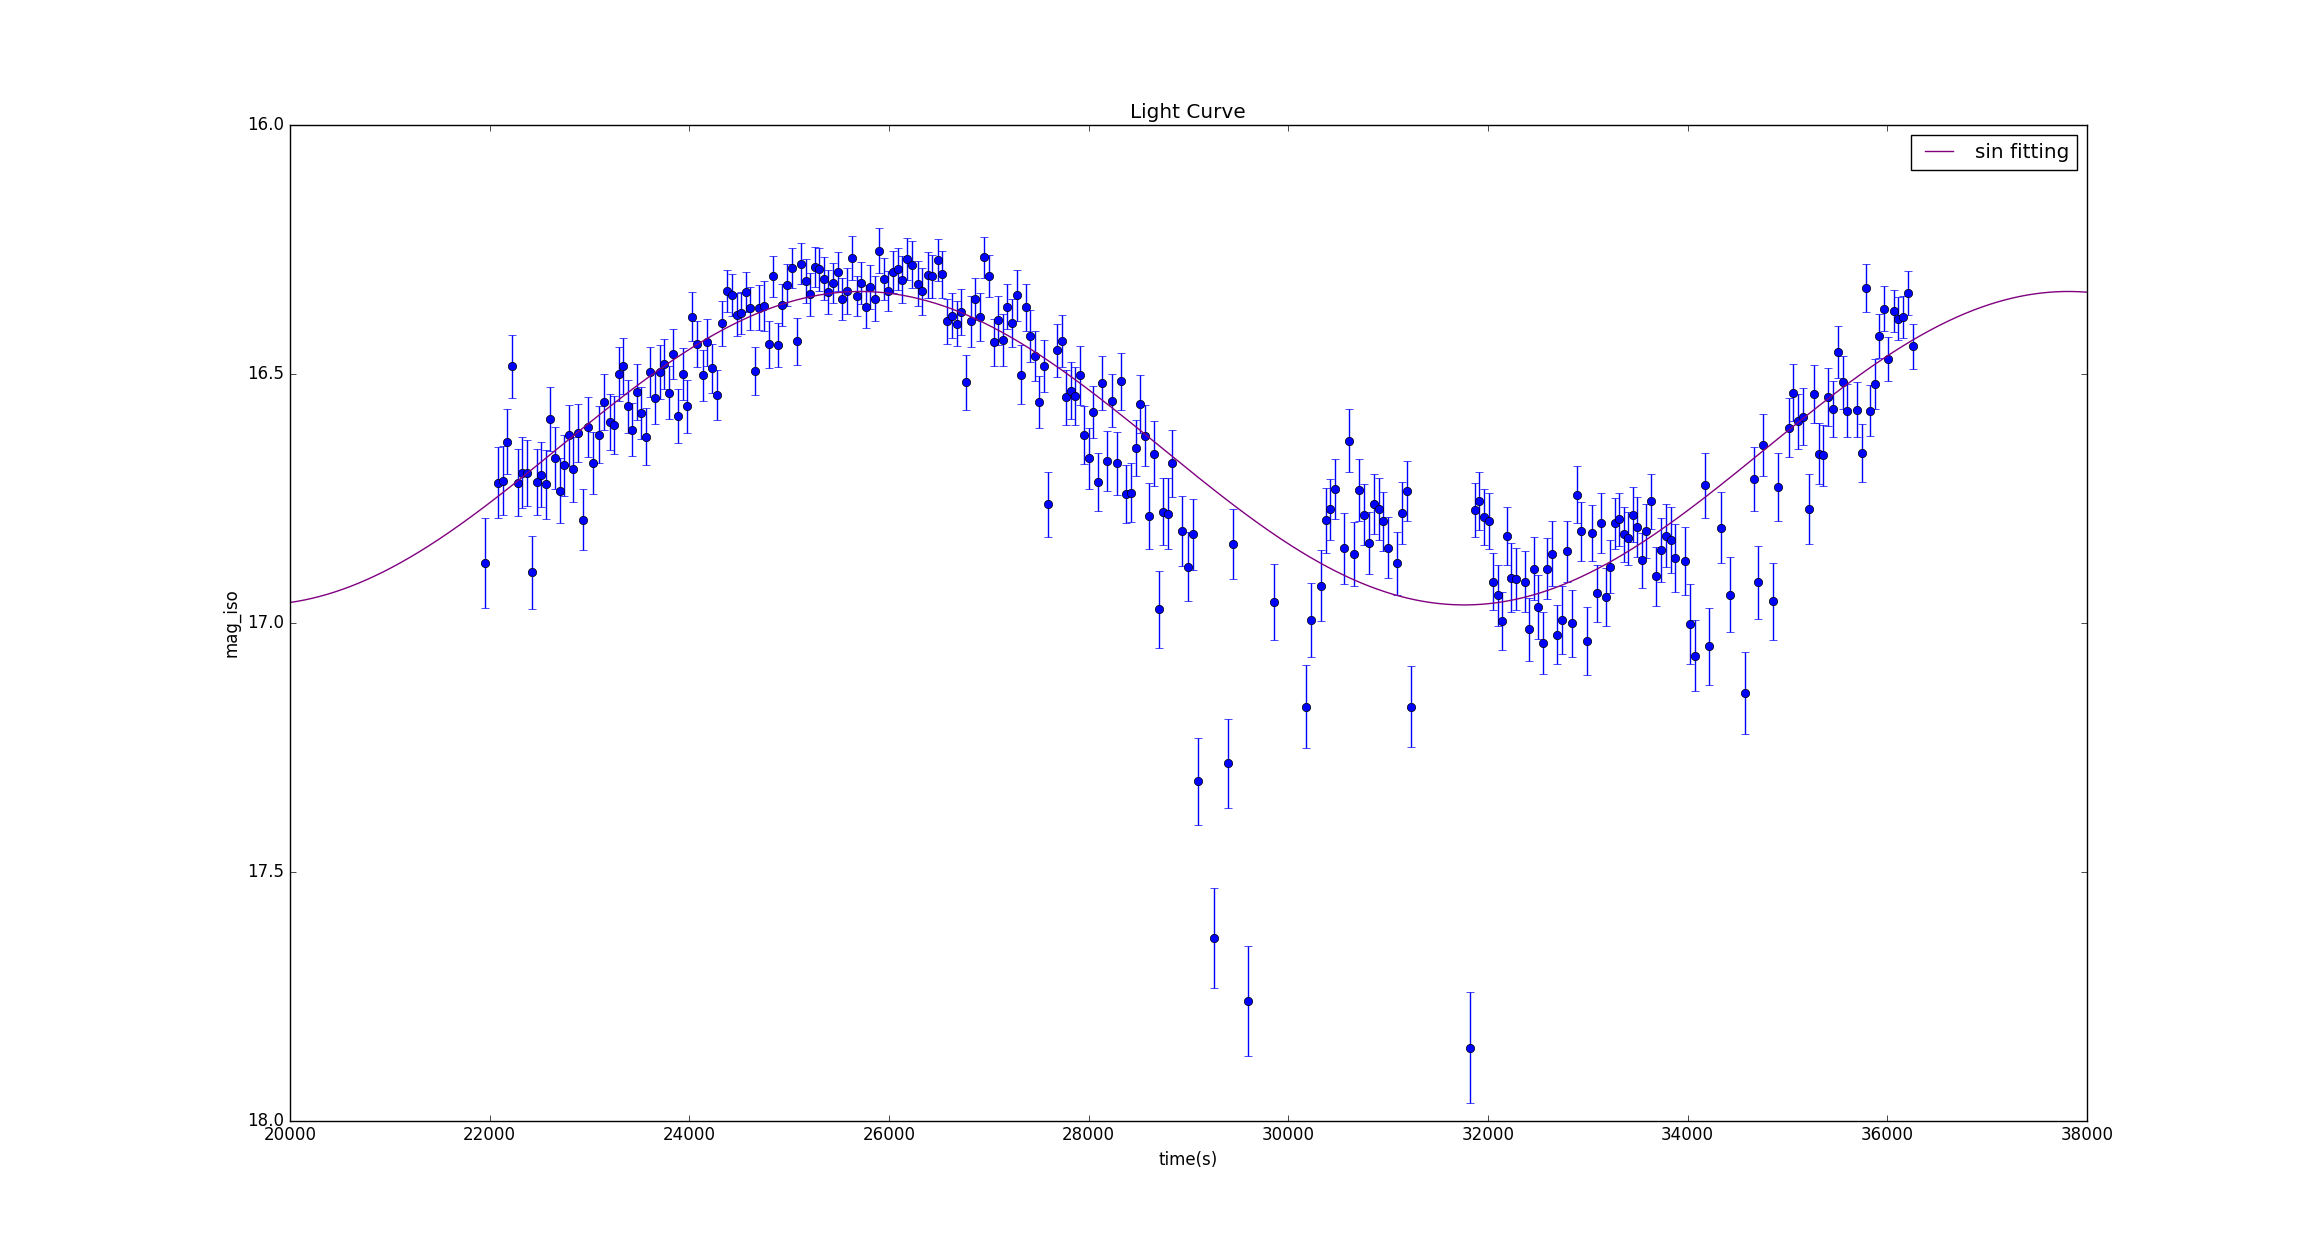
\includegraphics[scale=0.3]{fitted_plot.png}
\end{figure*}
\section{DATA and FITTING}
We select a photo that is relatively clear to do a calibration on the apparent magnitudes. For offset calibration, we first picked 15 stars on ds9 and match those on skymap.org, which gives us the right ascension and declination. Then in Simbad database, we can use those right ascension and declination to find the $MagB_{SIMBAD}$. We used it to calculate the magnitude's offset, which is shown on table 1.
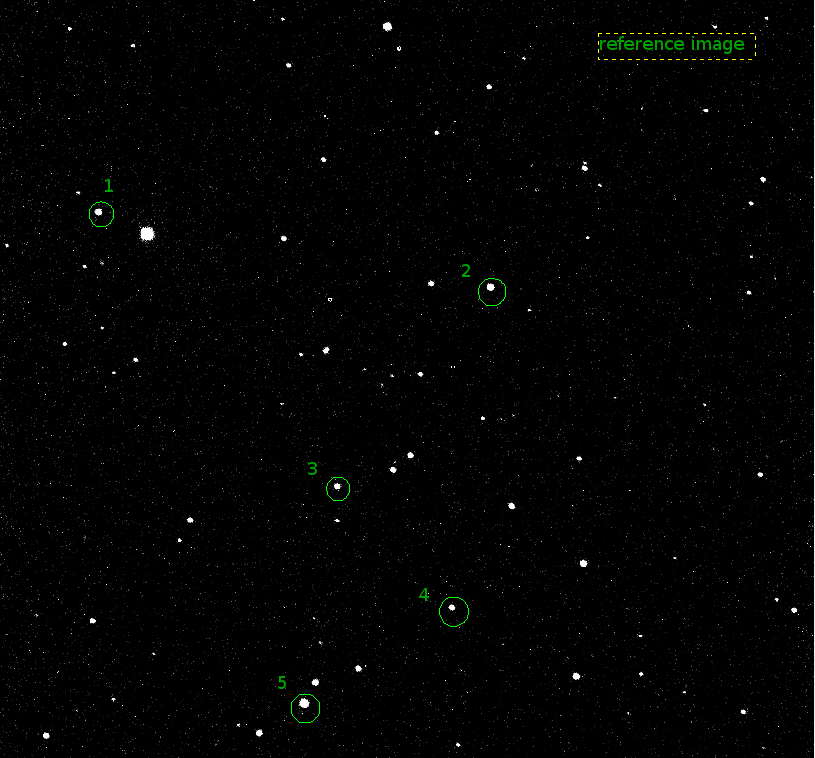
\includegraphics[scale=0.3]{reference_image.png}
For, scale calibration, we selected 5 stars as the figure shown above. Out of three hundred and five fits images, we were able to match these five stars to two hundred and fifty seven of images. Since they are at the constant position at the sky, we calculate the individual ratio of magnitude between each images to one of the image, and calibrated each image. 
\\The curve in the next page is a after calibration curve, where has a sine like relation. $$y=asin[wx+d]+c$$where the coefficients are in 95\% of confidence bound:
$$a=-0.3147\pm0.02035$$$$w=0.0005192\pm0.00001270$$$$d=0.7873\pm0.3695$$$$c=16.65\pm0.01500$$From the fit, we can calculate the period, $$T= \frac{2\pi}{w}=(12110\pm300) s$$On the other hand, the eclipse time is the region where the data has a much higher magnitude then that the rest. In the curve, there is a small region where the data looks disappeared, and that is the eclipse time we look for.
\begin{table}[h!]
\label{table:3}
\begin{tabular}{|c c c|}
\hline
Time average Apparent Magnitude & Orbital period (s)& Eclipse time (s)\\  [1 ex] \hline\hline
$16.65\pm0.01500$ & $12110\pm300$ & $\approx500$ \\ [1ex]\hline
\end{tabular}
\end{table}
 
\section{Method and Assumption}
NN Serpentis is a binary system with $e\approx10^{-3}$ [6]. So, it is a circular orbit, therefore, I assume $T=\frac{2\pi d}{v}$. Because of that, the ratio of the orbital period to the eclipse period is equal to the ratio of the circumference and the arc length that correspond to the eclipse. And since the NN Serpentis is very far away, the separation angle is small, here is another assumption $\delta s\approx2R_w$.
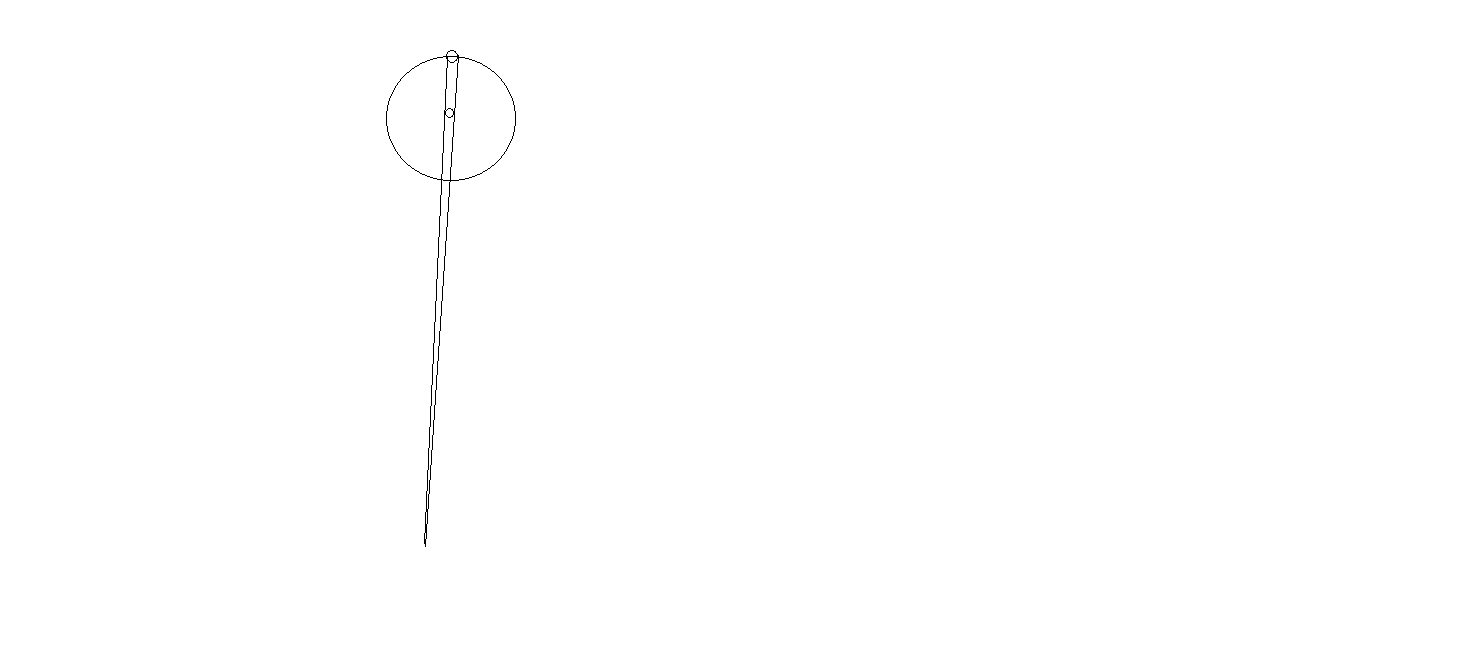
\includegraphics[scale=0.3]{image_2.png}
\begin{equation}
\frac{T}{t}=\frac{2\pi d}{\delta s}\approx\frac{2\pi d}{2R_w}
\end{equation}
\\ By combining equation (1),(6) and (7), $m_w$ can be calculated.
\begin{equation}
(\frac{\pi t}{T})^{3}=(\frac{R}{d})^{3}=\frac{4\pi^{2}}{74^{3}G}\frac{R_\odot^{3}M_\odot}{T^{2}m_w^{2}}
\end{equation}
\section{Calculation}
\subsection{Mass and radius of the white dwarf}
With the orbital period and the eclipse time, we can now calculate the mass of the white dwarf, which gives $$m_w\approx(0.03338\pm0.005935)M\odot$$Now, we can calculate the $R_w$ with equation (1).$$R_w\approx(0.04227\pm0.00253)R\odot$$

\subsection{Orbital radius}
Using equation (5),$$d\approx(0.3263\pm0.02756)R_\odot$$
\subsection{Distance from earth}
According to a online database from Kyoto Unviersity[5], the absolute  magnitude of NN Serpentis is $M=8.11$. Using equation (2), the distance from earth is $$r=(527.0\pm20.00)parsec$$



\section{Results}
Unfortunately, we cannot calculate the mass of the red dwarf and its radius by the magnitude-time relation. On the other hand, since I have made some assumptions, so it is important to make a comparison to other data base. In both table 3 and figure 1,2,3, there are some do not have the uncertainty and the error bars. That is because such errors are not displayed on those reference papers.
\\Unfortunately, only the result of eclipse time and the distance between earth and NN Serpentis agree to the reference. And the rest are mostly off by a few factor less than 3 except for mass, which off by a factor of 15.
\begin{table}[h!]
\centering
\caption{Comparison to other data base}
\begin{tabular}{||c c c ||} 
 \hline
 & our result & data from[5] and [6] \\ [1ex] 
 \hline\hline
 Apparent Magnitude & $ 16.65\pm0.01500 $ & 16.60\\
 Orbital Period(s) & $12110\pm300$ & 11239\\
 Eclipse time (s) & $\approx500$ & $480\pm36$ \\
 Mass & $(0.03338\pm 0.005935)M_\odot$ & $(0.535\pm0.012)M_\odot$ \\
 Radius& $(0.04227\pm0.00253)R_\odot$ & $(0.0211\pm0.0002)R_\odot$ \\
 orbital radius & $(0.3263\pm0.02756)R_\odot$ & $(0.934\pm0.0009)R_\odot$ \\
 distance (parsec) & $(527.0\pm20.00)$ & $(512\pm43)$\\
\hline\hline 
\end{tabular}
\label{table:1}
\end{table}
\begin{figure}
\centering
\caption{Apparent Magnitude;Orbital Period(s);Eclipse time(s)}
\begin{tikzpicture}
\begin{axis} [log ticks with fixed point
,symbolic x coords={1,2},width=3.5cm,height=8cm,xtick=data,ytick=data]
\addplot+[only marks] plot[error bars/.cd, y dir=both, y explicit]
coordinates{
    (1,16.65) +- (0.015,0.015)
    (2,16.60) +- (0,0) 
};
\end{axis}
\end{tikzpicture}
\begin{tikzpicture}
\begin{axis} [log ticks with fixed point
,symbolic x coords={1,2},width=3.5cm,height=8cm,xtick=data,ytick=data]
\addplot+[only marks] plot[error bars/.cd, y dir=both, y explicit]
coordinates{
    (1,12110) +- (300,300)
    (2,11239) +- (0,0) 
};
\end{axis}
\end{tikzpicture}
\begin{tikzpicture}
\begin{axis} [log ticks with fixed point
,symbolic x coords={1,2},width=3.5cm,height=8cm,xtick=data,ytick=data]
\addplot+[only marks] plot[error bars/.cd, y dir=both, y explicit]
coordinates{
    (1,500) +- (0,00)
    (2,480) +- (36.60,36.60) 
};
\end{axis}
\end{tikzpicture}
\end{figure}
\begin{figure}
\centering
\caption{Mass;Radius}
\begin{tikzpicture}
\begin{axis} [log ticks with fixed point
,symbolic x coords={1,2},width=3.5cm,height=8cm,xtick=data,ytick=data]
\addplot+[only marks] plot[error bars/.cd, y dir=both, y explicit]
coordinates{
    (1,0.0338) +- (0.005935,0.005935)
    (2,0.535) +- (0.012,0.012) 
};
\end{axis}
\end{tikzpicture}
\begin{tikzpicture}
\begin{axis} [log ticks with fixed point
,symbolic x coords={1,2},width=3.5cm,height=8cm,xtick=data,ytick=data]
\addplot+[only marks] plot[error bars/.cd, y dir=both, y explicit]
coordinates{
    (1,0.04227) +- (0.00253,0.00253)
    (2,0.0211) +- (0.0002,0.0002) 
};
\end{axis}
\end{tikzpicture}
\end{figure}
\begin{figure}
\centering
\caption{Orbital Radius; distance}
\begin{tikzpicture}
\begin{axis} [log ticks with fixed point
,symbolic x coords={1,2},width=3.5cm,height=8cm,xtick=data,ytick=data]
\addplot+[only marks] plot[error bars/.cd, y dir=both, y explicit]
coordinates{
    (1,0.3263) +- (0.02756,0.02756)
    (2,0.934) +- (0.0009,0.0009) 
};
\end{axis}
\end{tikzpicture}
\begin{tikzpicture}
\begin{axis} [log ticks with fixed point
,symbolic x coords={1,2},width=3.5cm,height=8cm,xtick=data,ytick=data]
\addplot+[only marks] plot[error bars/.cd, y dir=both, y explicit]
coordinates{
    (1,527.0) +- (20,20)
    (2,512) +- (43,43) 
};
\end{axis}
\end{tikzpicture}
\end{figure}




\section{Discussion}
Since I have made some crucial assumptions in equation (1) and (7), so the mass, the radius, as well as the orbital radius are an approximation. So the result of those physical quantities are excepted to be off by some factor. But the offset on the mass of the white dwarf is unexpected, so the method that I have been used in this paper is not suitable for a accurate calculation, but it can be applied as a rough pre-calculation for a similar system. Although it would be likely off by $10^{1}$, it gives an round idea of those quantity.  
On the other hand, the orbital period also does not agree with the actual value even with the consideration of uncertainty. This infers that a sine fit may not be the accurate fit our NN Serpentis.

\section{Future work}
For a more accurate approximation on each physical quantities, those assumptions should be re-examined, especially for equation (1).

\bibliography{bib}
\cite{lamport1994latex}
\footnotesize[2] Cutri, R. M.; et al. (2003). "2MASS All-Sky Catalog of Point Sources". VizieR On-line Data Catalog. 2246. 
\footnotesize[3] Phillips, A. C. (2010). The physics of stars. Chichester: John Wiley, Sons.
\footnotesize[4] Chromey, Frederick R. To Measure the Sky: an Introduction to Observational Astronomy. Cambridge University Press, 2016.
\footnotesize[5] $Yamashiki, Yosuke, et al. “NN Ser (AB).” NN Ser (AB), Kyoto Unviers-
ity, www.exoplanetkyoto.org/exohtml/NN_Ser_(AB).html.$
\footnotesize[6] Parsons, S. G.; Marsh, T. R.; Copperwheat, C. M.; Dhillon, V. S.; Littlefair, S. P.; Gänsicke, B. T.; Hickman, R. (2010). "Precise mass and radius values for the white dwarf and low mass M dwarf in the pre-cataclysmic binary NN Serpentis". Monthly Notices of the Royal Astronomical Society. 402 (4): 2591–2608.
\bibliographystyle{ieeetr}

\end{document}